\chapter{Background}

\section{Databases for FAU estimation}
The following datasets contain AU labels of subjects which are relevant to this work:

\begin{itemize}
    \item The DISFA database \cite{disfa}, which contains 27 subjects whose spontaneous
          facial expressions were captured in controlled recording conditions.
    \item CK+ \cite{Lucey2010} containing 123 subjects recorded with faces in strictly front positions.
    \item FERA 2015 BP4D-Spontaneous Dataset \cite{Valstar}:
          containing 41 subjects and 34 AUs, the subjects were young adults who
          spontaneously generated emotional responses to stimulus tasks.
\end{itemize}

This is just a small selection, however is it representative of the types of
datasets available. Each frame of the videos has a label which describes which AUs are
present and their intensity. Hence two distinct problems can be tackled here, intensity
estimation and classification, this work follows the classification route however
with neural networks it is potentially not a radically different problem.

A key challenge with these datasets is that they often have very unbalanced and
sparse labels as shown in figure \ref{disfastats}. This calls for methods
to balance training samples with respect to this imbalance and is the
motivation for using some unsupervised learning techniques, in order to extract information
from the unlabelled data.

A further two datasets are the TFD and SEMAINE, these do not contain AUs but often crop up in the
literature:
\begin{itemize}
     \item TFD \cite{tfd} Toronto Face Dataset
     \item The SEMAINE \cite{semaine} corpus which contains recordings
           of people interacting with a Sensitive Artificial Listener (SAL) in controlled conditions.
\end{itemize}

\section{The DISFA dataset} \label{disfa_list}
The Denver Intensity of Spontaneous Facial Action Dataset (DISFA)
of central interest to the project is the DISFA dataset \cite{disfa}, it is a set
of videos of people watching 9 short clips from youtube which try to span a range
of emotions such as emotions happiness, surprise, fear, disgust and sadness. Included
are 27 subjects with 12 AUs.

Each frame in each subject video has a label which quantifies how much of each
AU is present on a scale of 0-5, the distribution of intensities is shown in table \ref{compau}.

A challenge of the DISFA dataset is that it has many frames which are unlabelled, this is demonstrated
per subject in figure \ref{disfastats}. Many of the subjects have over 40\% of their frames unlabelled
, one outlier has over 75\% unlabelled.

\begin{table}[h!]
\centering

\begin{tabular}{lllllll}
\hline
Intensity & 0      & 1     & 2     & 3     & 4    & 5    \\ \hline
AU1       & 112286 & 2272  & 1749  & 2809  & 1393 & 555  \\
AU2       & 99165  & 1720  & 934   & 3505  & 836  & 369  \\
AU4       & 106160 & 4661  & 7636  & 6586  & 4328 & 1383 \\
AU5       & 99015  & 1579  & 719   & 293   & 104  & 34   \\
AU6       & 106425 & 9157  & 5986  & 3599  & 601  & 141  \\
AU9       & 99458  & 1659  & 2035  & 3045  & 316  & 77   \\
AU12      & 99987  & 13943 & 6869  & 7233  & 2550 & 172  \\
AU15      & 108358 & 5180  & 1618  & 1017  & 47   & 0    \\
AU17      & 117824 & 6342  & 4184  & 2281  & 112  & 11   \\
AU20      & 121377 & 1591  & 1608  & 1305  & 28   & 0    \\
AU25      & 84721  & 9805  & 13935 & 15674 & 5580 & 1039 \\
AU26      & 105778 & 13443 & 7473  & 3529  & 314  & 217  \\ \hline
\end{tabular}
\caption{A comparison of the number of occurrences of each intensity for each AU in the DISFA dataset. Note the total number
of AUs tabled here is larger than the number of frames, this is because some frames have multiple AUs present.} \label{compau}
\end{table}


\begin{figure}[h!]
  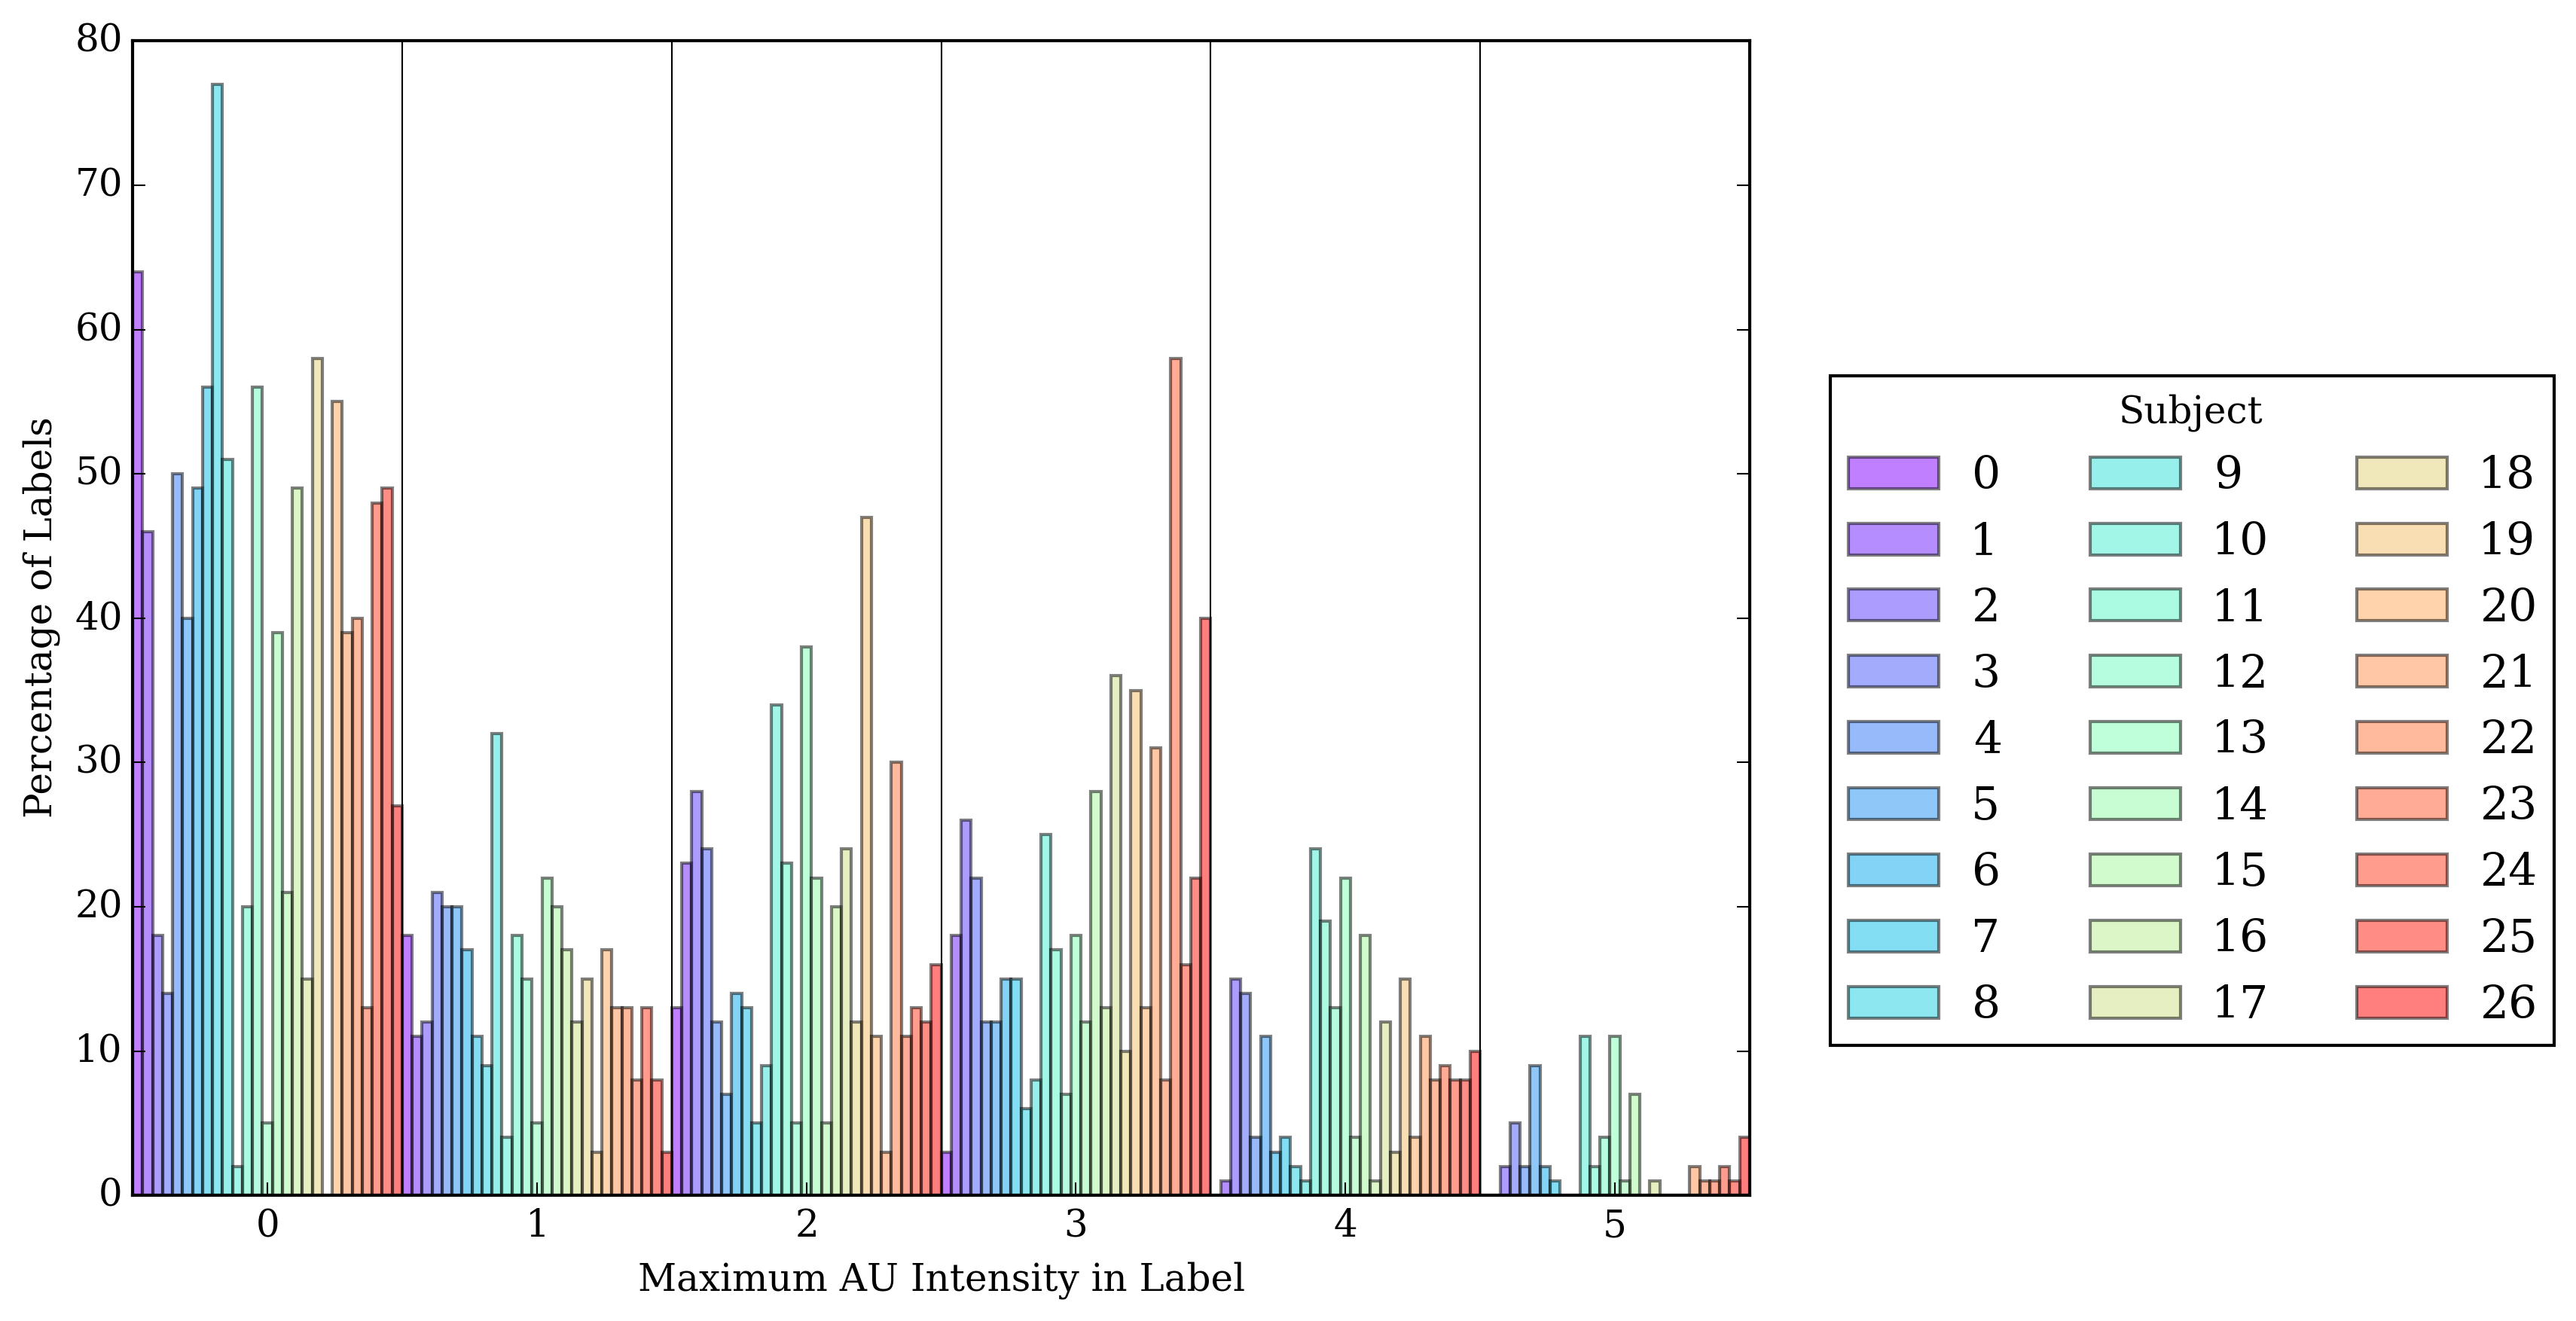
\includegraphics[width=\textwidth]{../graphs/maximum_label_intensity_disfa.pdf}
  \caption{DISFA dataset: This graph shows what the maximum value in each label is in the DISFA dataset per subject. This
  is done to illustrate the number of labels which contain very little information
  and pose an issue for a typical neural network structure. It also shows some there
  is quite a large degree of variation between subjects. In this work, frames are often refered to as unlabelled or neutral,
  in the figure this is all labels with maximum intensity zero.}\label{disfastats}
\end{figure}
\newpage

\section{Deep learning approaches to FAU detection}
It has been shown that deep neural networks containing convolutional, max pooling,
dropout and fully connected layers can effectively learn how to classify AUs in
a selection of datasets even when ignoring the temporal structure of the data \cite{Gudi2015,Ghosh2015,dodeeplearn}. These
Using the temporal data is also a possibily \cite{emonet,Jaiswal2016}.
%
%
%
\subsection*{Comparison of networks in Table \ref{tab:compnet}}
Network \cite{Ghosh2015} (Ghosh et al.) was trained on CK+, DISFA and BP4D datasets.
A key result of this paper was that they achieved good generalisation between datasets
with classifications accuracies between 60\% and 80\% for these generalisation experiments.
A feature particular to this network was that after the softmax layer, which assigns probabilities
to each AU it uses QDA (Quadratic Discriminant Analysis\cite{precogbook})  to
make predictions about whether AUs are present. A point of interest is also that
mean face normalisation is done per subject and then all for all subjects.

Network \cite{Gudi2015} (Amogh Gudi et al.) was trained on BP4D and SEMAINE
datasets achieving an average F1 score of 0.52 and 0.34 respectively. This paper
uses minimal preprocessing hence is a good example of how CNNs can learn features
with little feature engineering.

Network \cite{dodeeplearn} (Pooya Khorrami et al.) was trained on TFD and CK+,
this got average accuracies of 89.9\% and 98.3\% respectively in detecting emotions. This
is therefore not directly comparable, but they do explore connecting it with AUs.
An interesting point about this work is that they could stimulate activations in the convolutional
layers and directly see that the network had learned different facial actions demonstrating the
power of these networks.

Network \cite{Jaiswal2016} (Shashank Jaiswal et al.) was trained on SEMAINE and
BP4D achieving an overall weighted F1 score of 0.54. Which is on average higher
than network \cite{Gudi2015} as claimed in the paper. This paper includes a lot more
prior knowledge than the others, firstly it uses a BLSTM to incorporate temporal structure
and it defines multiple input streams from each facial region, allowing the convolutional
filters to become more specialised. This is the only paper where they say they use
two outputs for each AU so that the softmax creates a probability distribution for
each AU and not for all of them at once.

It should be noted that it is difficult to compare the performance between these
networks as they all use different evaluation scores as shown in table \ref{compscore}.
\begin{landscape}
\begin{table}[h!]
% \centering
{\footnotesize
\begin{tabular}{|lllllllll|}
\hline
Network                      & \multicolumn{2}{c}{Ghosh et. al\cite{Ghosh2015}}                         & \multicolumn{2}{c}{Gudi et. al.\cite{Gudi2015}}                            & \multicolumn{2}{c}{Khorrami et. al.\cite{dodeeplearn}}                          & \multicolumn{2}{c|}{Jaiswal et. al.\cite{Jaiswal2016}}   \\ \hline
\multicolumn{1}{|l|}{Element} & Type     & \multicolumn{1}{l|}{Dimensions}                    & Type     & \multicolumn{1}{l|}{Dimensions}                      & Type          & \multicolumn{1}{l|}{Dimensions}                  & Type      & Dimensions                     \\ \hline
\multicolumn{1}{|l|}{x}       &          & \multicolumn{1}{l|}{$40\times40\times1$}           &          & \multicolumn{1}{l|}{$48\times 48\times1$}            &               & \multicolumn{1}{l|}{$96\times96\times1$}         &           & $?\times?\times1$              \\ \hline
\multicolumn{1}{|l|}{$L_1$}   & conv 1   & \multicolumn{1}{l|}{$12\times 12\times1\times 70$} & conv 1   & \multicolumn{1}{l|}{$5\times 5\times1\times64$}      & conv 1        & \multicolumn{1}{l|}{$5\times5\times1\times64$}   & conv 1*   & $5\times5\times(2n+1)\times32$ \\
\multicolumn{1}{|l|}{$y_1$}   &          & \multicolumn{1}{l|}{$29\times29\times70$}          &          & \multicolumn{1}{l|}{$44\times44\times64$}            &               & \multicolumn{1}{l|}{$92\times92\times64$}        &           & $?\times?\times32$             \\ \hline
\multicolumn{1}{|l|}{$L_2$}   & max pool & \multicolumn{1}{l|}{$2\times 2$}                   & max pool & \multicolumn{1}{l|}{$3\times3$ (stride 2)}           & max pool      & \multicolumn{1}{l|}{$2\times2$}                  & max pool*  & $3\times3$                    \\
\multicolumn{1}{|l|}{$y_2$}   &          & \multicolumn{1}{l|}{$15\times15\times 70$}         &          & \multicolumn{1}{l|}{$22\times 22\times64$}           &               & \multicolumn{1}{l|}{$46\times46\times64$}        &           & $?\times?\times32$             \\ \hline
\multicolumn{1}{|l|}{$L_3$}   & conv 2   & \multicolumn{1}{l|}{$4\times 4\times70\times 10$}  & conv 2   & \multicolumn{1}{l|}{$5 \times 5 \times 64\times64$}  & conv 2        & \multicolumn{1}{l|}{$5\times5\times64\times128$} & conv 2    & $5\times5\times32\times64$     \\
\multicolumn{1}{|l|}{$y_3$}   &          & \multicolumn{1}{l|}{$12\times 12 \times 10$}       &          & \multicolumn{1}{l|}{$18 \times 18\times64$}          &               & \multicolumn{1}{l|}{$42\times42\times128$}       &           & $?\times?\times64$             \\ \hline
\multicolumn{1}{|l|}{$L_4$}   & max pool & \multicolumn{1}{l|}{$2\times 2$}                   & conv 3   & \multicolumn{1}{l|}{$4\times 4 \times64 \times 128$} & max pool      & \multicolumn{1}{l|}{$2\times2$}                  & conv 3    & $5\times5\times64\times64$     \\
\multicolumn{1}{|l|}{$y_4$}   &          & \multicolumn{1}{l|}{$6\times 6 \times 12$}         &          & \multicolumn{1}{l|}{$15\times15\times128$}           &               & \multicolumn{1}{l|}{$21\times21\times128$}       &           & $?\times?\times64$             \\ \hline
\multicolumn{1}{|l|}{$L_5$}   & fc       & \multicolumn{1}{l|}{$500$}                         & fc       & \multicolumn{1}{l|}{$3072$}                          & conv 3        & \multicolumn{1}{l|}{$5\times5\times1\times256$}  & conv 3    & $4\times4\times64\times128$    \\
\multicolumn{1}{|l|}{$y_5$}   &          & \multicolumn{1}{l|}{$500$}                         &          & \multicolumn{1}{l|}{$3072$}                          &               & \multicolumn{1}{l|}{$17\times17\times256$}       &           & $?\times?\times128$            \\ \hline
\multicolumn{1}{|l|}{$L_6$}   & fc       & \multicolumn{1}{l|}{$100$}                         & softmax  & \multicolumn{1}{l|}{$12$}                            & quadrant pool & \multicolumn{1}{l|}{}                            & fc        & $3072$                         \\
\multicolumn{1}{|l|}{$y_6$}   &          & \multicolumn{1}{l|}{$100$}                         &          & \multicolumn{1}{l|}{$12$}                            &               & \multicolumn{1}{l|}{$4\times4\times256$}         &           & $3072$                         \\ \hline
\multicolumn{1}{|l|}{$L_7$}   & softmax  & \multicolumn{1}{l|}{$12$}                          &          & \multicolumn{1}{l|}{}                                & fc            & \multicolumn{1}{l|}{$300$}                       & softmax   & $2N_{C}$                       \\
\multicolumn{1}{|l|}{$y_7$}   &          & \multicolumn{1}{l|}{$12$}                          &          & \multicolumn{1}{l|}{}                                &               & \multicolumn{1}{l|}{$300$}                       &           & $2N_{C}$                       \\ \hline
\multicolumn{1}{|l|}{$L_8$}   & QDA      & \multicolumn{1}{l|}{}                              &          & \multicolumn{1}{l|}{}                                & softmax       & \multicolumn{1}{l|}{$8$}                         & BLSTM     &                                \\
\multicolumn{1}{|l|}{$y_8$}   &          & \multicolumn{1}{l|}{}                              &          & \multicolumn{1}{l|}{}                                &               & \multicolumn{1}{l|}{$8$}                         &           &                                \\ \hline
\end{tabular}

\caption{A comparison of network architectures from the literature, all networks
use RELUs as their activation functions apart from in the final layer where it is
typical to use a softmax. $x$ denotes the input image, $L_i$ denotes the $i$th layer and $y_i$ denotes the output of the $i$th layer.
$N_{C}$ is the number of classes.
The question marks signify the dimensions of input images are variable as it depends on the input stream. fc is for fully connected and
conv is for a convolutional layer. QDA is Quadratic Discriminant Analysis and BLSTM is for Bidirectional Long Short-Term Memory neural
networks.
\newline
*These layers are per input stream} \label{tab:compnet}

}
\end{table}
\end{landscape}
\begin{table}[h!]
\centering

\begin{tabular}{lcccc}
\hline
Score    & \multicolumn{1}{l}{Ghosh et. al\cite{Ghosh2015}} & \multicolumn{1}{l}{Gudi et. al.\cite{Gudi2015}} & \multicolumn{1}{l}{Khorrami et. al.\cite{dodeeplearn}} & \multicolumn{1}{l}{Jaiswal et. al.\cite{Jaiswal2016}} \\ \hline
Accuracy & \checkmark                                       &                                                 & \checkmark                                             &                                             \\
F1       &                                                  & \checkmark                                      &                                                        & \checkmark                                  \\
AUC      &                                                  &                                                 &                                                        &                                             \\
2AFC     & \checkmark                                       & \checkmark                                      &                                                        &                                             \\ \hline
\end{tabular}
\caption{A comparison of which evaluation methods were used in the relevant papers.} \label{compscore}
\end{table}

\begin{table}[h!]
\centering

\begin{tabular}{lcccc}
\hline
Dataset    & \multicolumn{1}{l}{Ghosh et. al\cite{Ghosh2015}} & \multicolumn{1}{l}{Gudi et. al.\cite{Gudi2015}} & \multicolumn{1}{l}{Khorrami et. al.\cite{dodeeplearn}} & \multicolumn{1}{l}{Jaiswal et. al.\cite{Jaiswal2016}} \\ \hline
CK+      & \checkmark                            &                                      &                                         & \checkmark                              \\
DISFA    & \checkmark                            &                                      &                                         &                                         \\
SEMAINE* &                                       & \checkmark                           & \checkmark                              &                                         \\
BP4D*    & \checkmark                            & \checkmark                           & \checkmark                              &                                         \\
TFD      &                                       &                                      &                                         & \checkmark                              \\ \hline
\end{tabular}
\caption{A comparison of which datasets were used in the relevant papers.} \label{compdat}
\end{table}


%
%
%
